\begin{figure}[H]
\centering
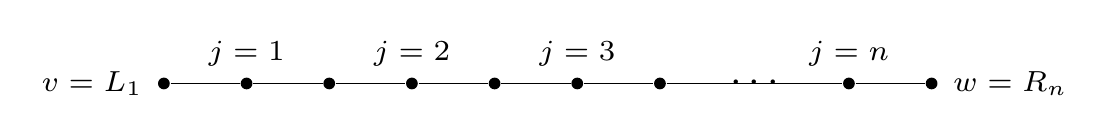
\begin{tikzpicture}[
scale=1.5,
transform shape,
point/.style={circle, fill=black, inner sep=1pt}
]

% vertices
\node[point, label=left:{\scriptsize $v=L_1$}] (v) at (0,0) {};
\node[point] (m1) at (0.7,0) {};
\node[point] (r1) at (1.4,0) {};

\node[point] (m2) at (2.1,0) {};
\node[point] (r2) at (2.8,0) {};

\node[point] (m3) at (3.5,0) {};
\node[point] (r3) at (4.2,0) {};

\node at (5.0,0) {$\cdots$};

\node[point] (mn) at (5.8,0) {};
\node[point, label=right:{\scriptsize $w=R_n$}] (rn) at (6.5,0) {};

% edges
\draw (v) -- (m1) -- (r1) -- (m2) -- (r2) -- (m3) -- (r3);
\draw (r3) -- (mn) -- (rn);

% gadget labels
\node at (0.7,0.25) {\scriptsize $j=1$};
\node at (2.1,0.25) {\scriptsize $j=2$};
\node at (3.5,0.25) {\scriptsize $j=3$};
\node at (5.8,0.25) {\scriptsize $j=n$};

\end{tikzpicture}
\caption{$n$ multi-party disjointness gadgets chained together.}
\label{fig:multi-disj-chain}
\end{figure}